
%====================================================================
\chapter{Operations Within the Enclave}
\label{sec:Enclave}
%====================================================================

A number of interactions with TIS may occur within the
Enclave.
These interactions leave some of the $IDStation$ state unchanged.

\begin{schema}{EnclaveContext}
        \Delta IDStation
\\      RealWorldChanges
\also
        \Xi TISControlledRealWorld
\also
        \Xi UserToken
\\      \Xi AdminToken
\\      \Xi Finger
\\      \Xi Stats
\where
        tokenRemovalTimeout' = tokenRemovalTimeout
\end{schema}
\begin{Zcomment}
\item
The following state components may change $KeyStore$, 
$Floppy$, $Config$, $Admin$, $Keyboard$,
$DoorLatchAlarm$, $Internal$ and $AuditLog$. 
\item
The components of the real world controlled by TIS remain unchanged.
\end{Zcomment}

The operations that may occur within the enclave include
administrator operations and the ID station enrolment. These are
described in this section.

%-------------------------------------------------------------------------
\section{Enrolment of an ID Station}
%-------------------------------------------------------------------------

\begin{traceunit}{FS.Enclave.TISEnrolOp}
\end{traceunit}

Before TIS can be used it must be enrolled.

We assume
that the initial enrolment is the only possible enrolment activity.

Enrolment is a multi-phase activity, the state transistions for an
enrolment are given in Figure \ref{fig:enrol}. Before enrolment the
system is in state $notEnrolled$ and, on successful completion, it
enters the $quiescent$ state.

\begin{figure}[htbp]
  \begin{center}
    \leavevmode
    \resizebox{\textwidth}{!}{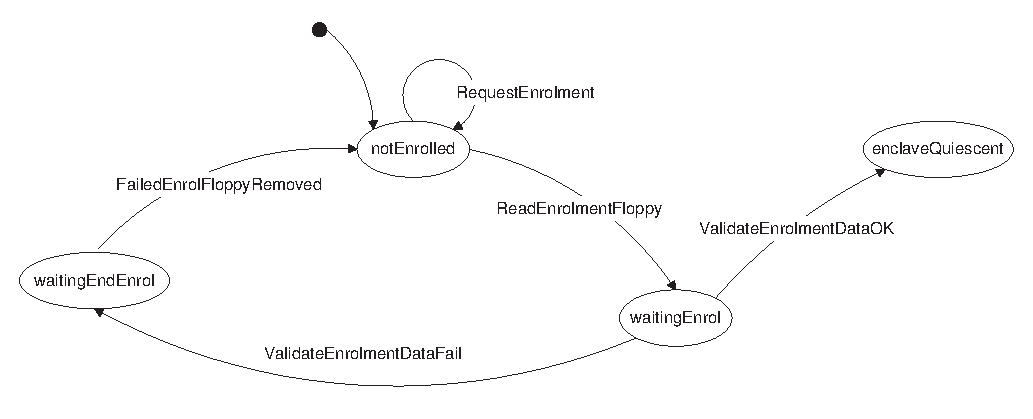
\includegraphics{41_2_enrol.eps}}
    \caption{Enrolment state transitions}
    \label{fig:enrol}
  \end{center}
\end{figure}

The context for all enrolment operations is given below.

\begin{schema}{EnrolContext}
        EnclaveContext
\also
        \Xi Keyboard
\\      \Xi Admin
\\      \Xi DoorLatchAlarm
\\      \Xi Config
\\      \Xi Floppy
\end{schema}

\begin{Zcomment}
\item
The following state components may change
$KeyStore$, $Internal$ and $AuditLog$. 
\end{Zcomment}


%...................................
\subsection{Requesting Enrolment}
%...................................

\begin{traceunit}{FS.Enclave.RequestEnrolment}
\end{traceunit}


The ID station will request enrolment while there is no Floppy
present. This will occur until a successful enrolment is achieved.

\begin{schema}{RequestEnrolment}
        EnrolContext
\also
        \Xi KeyStore
\\      \Xi AuditLog
\\      \Xi Internal
\where
        enclaveStatus = notEnrolled
\\      floppyPresence = absent
\also
        currentScreen'.screenMsg = insertEnrolmentData
\also
        currentDisplay' = blank
\end{schema}

\begin{traceunit}{FS.Enclave.ReadEnrolmentFloppy}
\traceto{ScStart.Ass.Data}
\traceto{ScStart.Con.NoInterleave}
\end{traceunit}

If a floppy is present then TIS goes on to validate the
contents. Nothing is written to the log at this stage as log entries
will be made on successful or failed enrolment.

\begin{schema}{ReadEnrolmentFloppy}
        EnrolContext
\also
        \Xi KeyStore
\where
        enclaveStatus = notEnrolled
\\      floppyPresence = present
\also
        currentScreen'.screenMsg = validatingEnrolmentData 
\also
        enclaveStatus' = waitingEnrol     
\\      status' = status
\\      currentDisplay' = blank                         
\end{schema}

\begin{zed}
        ReadEnrolmentData \defs ReadEnrolmentFloppy \lor RequestEnrolment
\end{zed}

%.........................................
\subsection{Validating Enrolment data from Floppy}
%.........................................

For the enrolment data to be acceptable the data on the floppy must be
valid enrolment data with the ID Station certificate containing this
ID station's public key. 

\begin{schema}{EnrolmentDataOK}
        Floppy
\\      KeyStore
\where
        currentFloppy \in \ran enrolmentFile
\\      (\exists ValidEnrol @ \theta ValidEnrol = enrolmentFile \inv
currentFloppy)
\end{schema}

\begin{traceunit}{FS.Enclave.ValidateEnrolmentDataOK}
\traceto{ScStart.Suc.Running}
\traceto{ScStart.Suc.Audit}
\traceto{FMT\_MSA.2.1}
\traceto{FMT\_MTD.3.1}
\end{traceunit}


If the data on the floppy is acceptable to be used for enrolment then
the Key store is updated. From this point the system is available for
use both by users entering the enclave and by administrators.

\begin{schema}{ValidateEnrolmentDataOK}
        EnrolContext
\also
        UpdateKeyStoreFromFloppy
\\      AddElementsToLog
\where
        enclaveStatus = waitingEnrol
\also
        EnrolmentDataOK
\also
        currentScreen'.screenMsg = welcomeAdmin
\also
        enclaveStatus' = enclaveQuiescent 
\\      status' = quiescent
\\      currentDisplay' = welcome
\end{schema}

\begin{traceunit}{FS.Enclave.ValidateEnrolmentDataFail}
\traceto{ScStart.Fail.ReadFloppy}
\end{traceunit}

If the enrolment fails then TIS waits for the floppy to be removed
before prompting for new enrolment data. 

\begin{schema}{ValidateEnrolmentDataFail}
        EnrolContext
\also
        \Xi KeyStore
\also
        AddElementsToLog
\where
        enclaveStatus = waitingEnrol
\also
        \lnot EnrolmentDataOK
\also
        currentScreen'.screenMsg = enrolmentFailed
\also
        enclaveStatus' = waitingEndEnrol
\\      status' = status
\\      currentDisplay' = blank
\end{schema}

\begin{zed}
        ValidateEnrolmentData \defs ValidateEnrolmentDataOK \lor
          ValidateEnrolmentDataFail
\end{zed}

%.........................................
\subsection{Completing a failed Enrolment}
%.........................................

A failed enrolment will only terminate once the floppy has been
removed, otherwise the system would repeatedly try to validate the
same floppy.

\begin{traceunit}{FS.Enclave.FailedEnrolFloppyRemoved}
\end{traceunit}


Once the floppy has been removed the administrator is prompted for
enrolment data again. We do not log the removal of the floppy in the
audit log.

\begin{schema}{FailedEnrolFloppyRemoved}
        EnrolContext
\also
        \Xi KeyStore
\where
        enclaveStatus = waitingEndEnrol
\\      floppyPresence = absent
\also
        currentScreen'.screenMsg = insertEnrolmentData
\also
        enclaveStatus' = notEnrolled
\\      status' = status
\\      currentDisplay' = blank
\end{schema}

\begin{traceunit}{FS.Enclave.WaitingFloppyRemoval}
\end{traceunit}

TIS will wait indefinately for the floppy to be removed after an
unsuccessful enrolment, this is because enrolment is triggered by the
presence of the floppy alone.

\begin{schema}{WaitingFloppyRemoval}
        EnclaveContext
\also
        \Xi IDStation
\where
        enclaveStatus = waitingEndEnrol
\\      floppyPresence = present
\end{schema}

\begin{zed}
        CompleteFailedEnrolment \defs FailedEnrolFloppyRemoved  
         \lor WaitingFloppyRemoval
\end{zed}

%..........................................
\subsection{The Complete Enrolment}
%..........................................

The complete enrolment process involves reading the enrolment data,
validating it and, in the case of a failure waiting for the system to
be in a state where it can try another enrolment.

\begin{zed}
        TISEnrolOp \defs ReadEnrolmentData \lor
ValidateEnrolmentData 
\\      \t4 \lor CompleteFailedEnrolment
\end{zed}

%-----------------------------------------------------------------------
\section{Administrator Token Tear}
%-----------------------------------------------------------------------

The action of removing the administrator Token will result in the
administrator being logged out of the system.

This may happen at any point once a token has been inserted into the
reader. As soon as the adminitrator's token is torn this action will
be logged. The screen message will be reset if the system is not busy
with processing a user entry.

\begin{schema}{AdminTokenTear}
         EnclaveContext
\also
        \Xi Config
\\      \Xi Floppy
\\      \Xi Keyboard
\\      \Xi DoorLatchAlarm
\\      \Xi KeyStore
\\      ResetScreenMessage
\where
        adminTokenPresence = absent
\also   
        status' = status
\\      currentDisplay' = currentDisplay
\also
        enclaveStatus' = enclaveQuiescent
\end{schema}

If the admin token is torn while the system is processing an activity
within the enclave then the activity will be stopped.

\begin{schema}{BadAdminTokenTear} 
        AdminTokenTear
\also
        AddElementsToLog
\where
        enclaveStatus \in \{gotAdminToken, waitingStartAdminOp, waitingFinishAdminOp \}
\end{schema}

\begin{traceunit}{FS.Enclave.BadAdminLogout}
\traceto{ScLogOff.Ass.LoggedOn}
\traceto{ScLogOff.Suc.LoggedOff}
\traceto{ScLogOff.Suc.Audit}
\end{traceunit}

If the administrator is performing an operation when the token is torn
then the administrator will be logged off.

\begin{schema}{BadAdminLogout}
        BadAdminTokenTear
\\      AdminLogout
\where
        enclaveStatus \in \{ waitingStartAdminOp, waitingFinishAdminOp
        \}
\end{schema}


\begin{traceunit}{FS.Enclave.LoginAborted}
\end{traceunit}

If the token is torn during the log on validation process then there
is no need to log off the administrator.

\begin{schema}{LoginAborted}
        BadAdminTokenTear
\\      \Xi Admin
\where
        enclaveStatus = gotAdminToken
\end{schema}


%----------------------------------------------------------------------
\section{Administrator Login}
%----------------------------------------------------------------------


An Administrator logs into TIS by inserting a valid token
into the $adminToken$ reader. The authorisation certificate is
verified and the user is logged in with the privileges indicated on
the card.

Once the administrator is successfully logged into TIS, the system
records that there is a role present. The process of logging on is
given by the state transition diagram in Figure \ref{fig:logon}

\begin{figure}[htbp]
  \begin{center}
    \leavevmode
    \resizebox{\textwidth}{!}{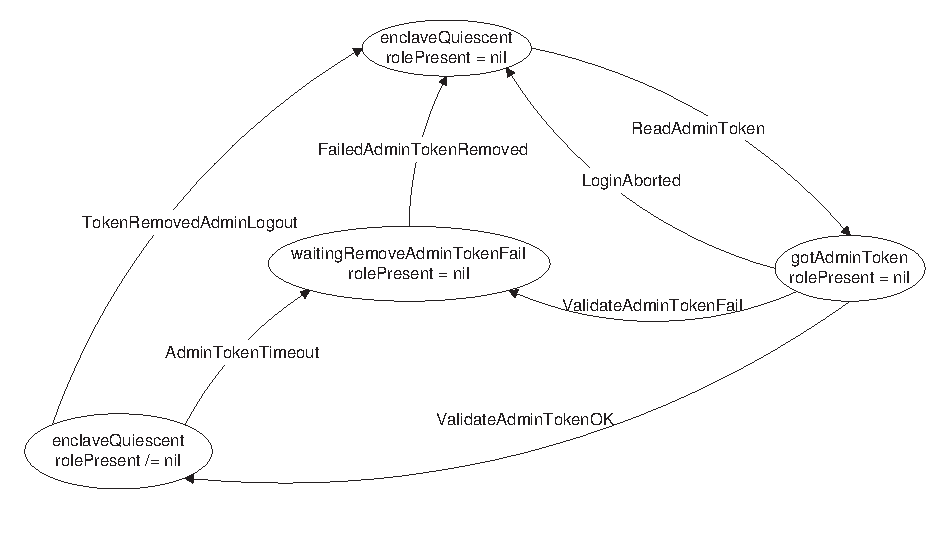
\includegraphics{41_2_admin.eps}}
    \caption{Administrator logon/logoff state transitions}
    \label{fig:logon}
  \end{center}
\end{figure}

The context for administrator login is given below.

\begin{schema}{LoginContext}
        EnclaveContext
\also
        \Xi Keyboard
\\      \Xi KeyStore
\\      \Xi DoorLatchAlarm
\\      \Xi Config
\\      \Xi Floppy
\where
        status' = status
\\      currentDisplay' = currentDisplay
\end{schema}

\begin{Zcomment}
\item
The following state components may change
$Admin$, $Internal$ and $AuditLog$. 
\end{Zcomment}

%..........................................
\subsection{Read Administrator Token}
%..........................................

\begin{traceunit}{FS.Enclave.ReadAdminToken}
\traceto{ScLogOn.Ass.Quiescent}
\traceto{ScLogOn.Suc.Audit}
\traceto{ScLogOn.Con.NoInterleave}
\traceto{FIA\_UID.2.1}
\traceto{FMT\_SMR.3.1}
\end{traceunit}

When the admin token is read the action is audited and the internal
status changes. No other aspects of the system are modified.

An administrator can only log on when there is no user entry activity
in progress or TIS is waiting for a failed user token to be removed
from the token reader outside of the enclave.

\begin{schema}{ReadAdminToken}
         LoginContext
\also
        \Xi Admin
\also
        AddElementsToLog
\where
        status \in \{~ quiescent, waitingRemoveTokenFail ~\}
\also
        enclaveStatus = enclaveQuiescent
\\      rolePresent = \Nil
\\	adminTokenPresence = present
\also
	enclaveStatus' = gotAdminToken
\\      currentScreen' = currentScreen
\end{schema}

The operation to read the token is as follows:

\begin{zed}
        TISReadAdminToken \defs 
                ReadAdminToken   
\end{zed}

%..........................................
\subsection{Validate Administrator Token}
%..........................................

An administrator's token is considered valid if it cotains a current
authorisation certificate that correctly cross references to the token
ID and the ID certificate and both these certificates can be validated
using the keys held in the $KeyStore$. Additionally the
privileges assigned to the user within the authorisation certificate
must indicate that the user is actually an administrator.

\begin{schema}{AdminTokenOK}
        AdminToken
\\      KeyStore
\\      currentTime : TIME        
\where
        currentAdminToken \in \ran goodT
\also
        \exists TokenWithValidAuth @
\\ \t1  (goodT(\theta TokenWithValidAuth )  = currentAdminToken
\\ \t1  \land (\exists IDCert @ \theta IDCert = idCert \land CertOK )
\\ \t1  \land (\exists AuthCert @ \theta AuthCert = \The authCert \land
AuthCertOK )
\\ \t1  \land (\The authCert).role \in ADMINPRIVILEGE 
\\ \t1  \land currentTime \in (\The authCert).validityPeriod)
\end{schema}
\begin{Zcomment}
\item
Only the $AuthCert$  and $IDCert$ are checked at this point. The remaining
certificates were checked on entry to the enclave.
\item
The Token must indicate that the user has an administrator privilege.
\end{Zcomment}

\begin{traceunit}{FS.Enclave.ValidateAdminTokenOK}
\traceto{ScLogOn.Ass.ValidAdmin}
\traceto{ScLogOn.Suc.LogOn}
\traceto{ScLogOn.Suc.Audit}
\traceto{SFP.DAC}
\traceto{FCO\_NRO.2.1}
\traceto{FCO\_NRO.2.2}
\traceto{FCO\_NRO.2.3}
\traceto{FDP\_ACC.1.1}
\traceto{FDP\_ACF.1.1}
\traceto{FDP\_ACF.1.2}
\traceto{FDP\_ACF.1.3}
\traceto{FDP\_ACF.1.4}
\traceto{FIA\_USB.1.1}
\traceto{FMT\_MSA.1.1}
\traceto{FMT\_MTD.1.1}
\traceto{FMT\_SAE.1.1}
\traceto{FMT\_SMR.2.1}
\traceto{FMT\_SMR.2.2}
\end{traceunit}


If the token can be validated then the administrator is logged onto
TIS.

\begin{schema}{ValidateAdminTokenOK}
        LoginContext
\also
        AdminLogon
\also
        AddElementsToLog
\where
        enclaveStatus = gotAdminToken
\\      adminTokenPresence = present
\also
        AdminTokenOK
\also   
        currentScreen'.screenMsg = requestAdminOp 
\also
        enclaveStatus' = enclaveQuiescent
\end{schema}

\begin{traceunit}{FS.Enclave.ValidateAdminTokenFail}
\traceto{ScLogOn.Fail.ReadCard}
\end{traceunit}

If the token can not be validated then TIS waits for it to be removed.

\begin{schema}{ValidateAdminTokenFail}
        LoginContext
\also
        \Xi Admin
\also
        AddElementsToLog
\where
        enclaveStatus = gotAdminToken
\\      adminTokenPresence = present
\also
        \lnot AdminTokenOK
\also
        currentScreen'.screenMsg = removeAdminToken
\also
        enclaveStatus' = waitingRemoveAdminTokenFail
\end{schema}

\begin{zed}
        TISValidateAdminToken \defs ValidateAdminTokenOK \lor
        ValidateAdminTokenFail 
\\ \t4  \lor
        LoginAborted
\end{zed}

\subsection{Complete Failed Administrator Logon}

If an administrator token has failed to be accepted by TIS 
then no further actions can take place in the enclave until it has 
been removed.

\begin{traceunit}{FS.Enclave.FailedAdminTokenRemoved}
\end{traceunit}


The administrator token may be removed at any point during a user
entry, hence the context for this
activity does not place restrictions on the value of $status$.

When the admin token is removed TIS returns to a state ready
to accept another administrator logon.
\begin{schema}{FailedAdminTokenRemoved}
        LoginContext
\also
        \Xi Admin
\also 
        AddElementsToLog
\where
        enclaveStatus = waitingRemoveAdminTokenFail
\\      adminTokenPresence = absent
\also
        currentScreen'.screenMsg = welcomeAdmin
\also
        enclaveStatus' = enclaveQuiescent
\also
        currentDisplay' = currentDisplay
\end{schema}

\begin{traceunit}{FS.Enclave.WaitingAdminTokenRemoval}
\end{traceunit}


TIS will wait indefinitely for the Admin Token to be removed after a
failed attempt to logon.

\begin{schema}{WaitingAdminTokenRemoval}
        EnclaveContext
\also
        \Xi IDStation
\where
        enclaveStatus = waitingRemoveAdminTokenFail
\\      adminTokenPresence = present     
\end{schema}

\begin{zed}
        TISCompleteFailedAdminLogon \defs FailedAdminTokenRemoved 
\lor WaitingAdminTokenRemoval
\end{zed}

\subsection{The Complete Administrator Logon}

\begin{traceunit}{FS.Enclave.TISAdminLogin}
\end{traceunit}

The complete administrator logon process, from the point that the
system has detected the presence of a token in the administrator
reader, involves 
validating the administrator token and, in the case of a failure 
waiting for the system to be in a state where it can try another logon.

\begin{zed}
        TISAdminLogon \defs TISReadAdminToken \lor TISValidateAdminToken \lor TISCompleteFailedAdminLogon
\end{zed}

%-----------------------------------------------------------------
\section{Administrator Logout}
%-----------------------------------------------------------------

Administrator logout can be achieved in two ways, either the
administrator removes their token from TIS, or the Authorisation
certificate on the token expires, causing the system to automatically
log off the administrator.

\begin{traceunit}{FS.Enclave.AdminLogout}
\traceto{ScLogOff.Ass.LoggedOn}
\traceto{ScLogOff.Suc.LoggedOff}
\traceto{ScLogOff.Suc.Audit}
\end{traceunit}

If TIS is not performing an administrator operation then the
token may be removed to log out the administrator.

\begin{schema}{TokenRemovedAdminLogout}
        AdminTokenTear
\\      AdminLogout
\also
        AddElementsToLog
\where
        enclaveStatus = enclaveQuiescent 
\\      rolePresent \neq \Nil
\end{schema}

\begin{traceunit}{FS.Enclave.AdminTokenTimeout}
\end{traceunit}


The TIS will automatically logout an administrator whose token
expires. This occurs if the validity period on the Authorisation
certificate expires.

\begin{schema}{AdminTokenTimeout}
        LoginContext
\also
        AdminLogout
\\      AddElementsToLog
\\      ResetScreenMessage
\where
        enclaveStatus = enclaveQuiescent 
\\      adminTokenPresence = present
\\      rolePresent \neq \Nil
\also
        \lnot AdminTokenOK
\also
        enclaveStatus' = waitingRemoveAdminTokenFail
\end{schema}

\begin{traceunit}{FS.Enclave.TISCompleteTimeoutAdminLogout}
\end{traceunit}

If the administrator's token expires then it must be removed before
further activities can take place at the TIS console. This behaviour
is identical to the behaviour when the system waits for a the
administrator to remove their token following a failed logon.

\begin{zed}
TISCompleteTimeoutAdminLogout \defs TISCompleteFailedAdminLogon
\end{zed}

%...........................
\subsection{Complete Administrator Logout}
%............................

\begin{traceunit}{FS.Enclave.TISAdminLogout}
\end{traceunit}

THe complete administrator logout process, from the point that it
decides to log out an administrator to the point that it is in a state
where it can try another logon is givien below.

\begin{zed}
TISAdminLogout \defs  TokenRemovedAdminLogout \lor AdminTokenTimeout \lor TISCompleteTimeoutAdminLogout 
\end{zed}

%-----------------------------------------------------------------
\section{Administrator Operations}
%-----------------------------------------------------------------
An administrator operation can take place as long as an administrator
is present. The operation is started by receiving a valid request to
perform an operation from the keyboard. TIS will ensure that the
requested operation is one compatible with the current role present.

Once the operation is started the behaviour depends on the type of
operation. Operations are either short, and can be implemented in one
phase or they are multi-phase operations. 

$shutdown$ and $overrideLock$ are short operations, while $archiveLog$
and $updateCofigData$ are multi phase operations.

The state transition diagram for administrator operations is given in
Figure \ref{fig:adminOp}

\begin{figure}[htbp]
  \begin{center}
    \leavevmode
    \resizebox{\textwidth}{!}{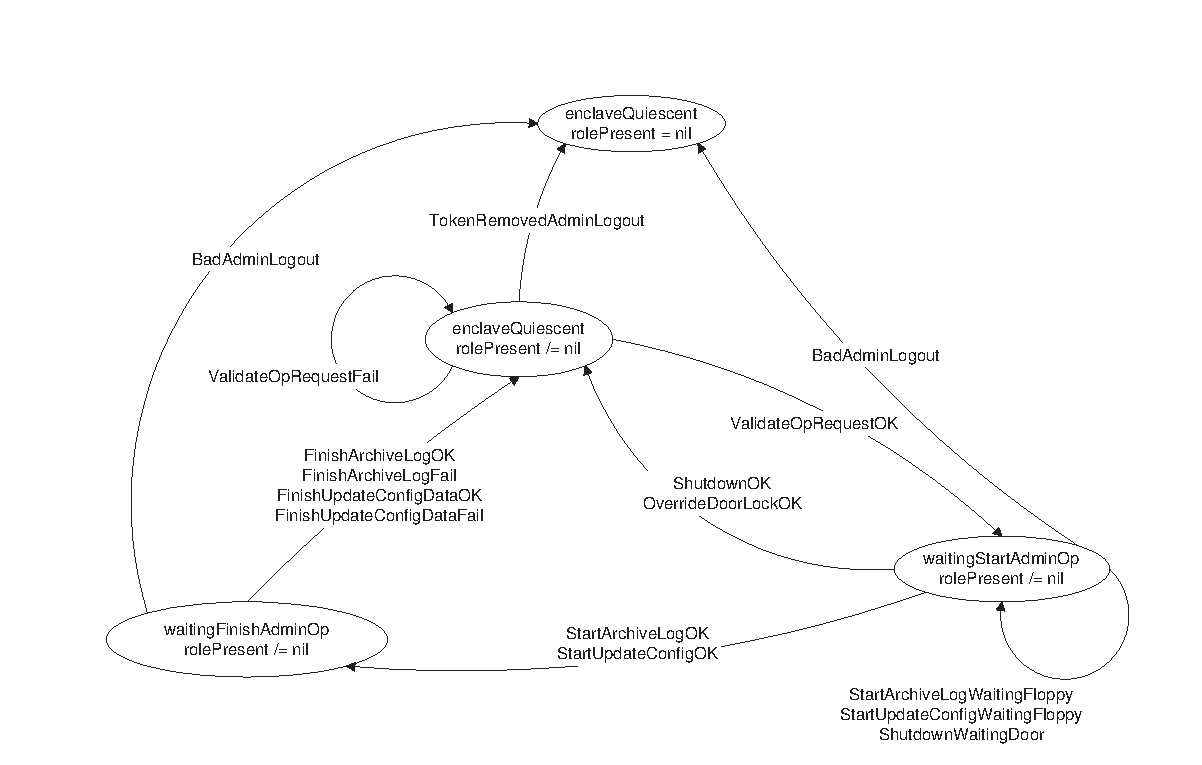
\includegraphics{41_2_adminOp.eps}}
    \caption{Administrator operation state transitions}
    \label{fig:adminOp}
  \end{center}
\end{figure}

All administrator operations have a common context, in which the
$AdminToken$ does not change.
An administrator can only perform an operation when there is no user 
entry activity
in progress or TIS is waiting for a failed user token to be removed
from the token reader outside of the enclave.


\begin{schema}{AdminOpContext}
        EnclaveContext
\also
        \Xi Keyboard
\\      \Xi KeyStore
\end{schema}
\begin{Zcomment}
\item
The following state components may change   
$Floppy$, $Config$, $Admin$, $DoorLatchAlarm$, $Internal$ and $AuditLog$. 
\end{Zcomment}

Once an operation has been started its context is given by:

\begin{schema}{AdminOpStartedContext}
        AdminOpContext
\where
        enclaveStatus = waitingStartAdminOp
\\      adminTokenPresence = present
\also
        status' = status
\end{schema}
\begin{Zcomment}
\item
The $adminToken$ will be present, its removal is erroneous.
\item
The system has a record of the name of the current operation.
\end{Zcomment}

Some operations are multi-phase, the context for completing a
multi-phase operation is given by: 

\begin{schema}{AdminOpFinishContext}
        AdminOpContext
\also
        AdminFinishOp
\where
        enclaveStatus = waitingFinishAdminOp
\\      adminTokenPresence = present
\also
        status' = status
\\      currentDisplay' = currentDisplay
\also
        enclaveStatus' = enclaveQuiescent
\end{schema}
\begin{Zcomment}
\item
The $adminToken$ will be present, its removal is erroneous.
\item
The enclaveStatus value implies that TIS has a record of the name of the
current operation from the $IDStation$ invariant.
\end{Zcomment}


%-----------------------------------------------------------------
\section{Starting Operations}
%-----------------------------------------------------------------



All administrator operations are initiated in the same way. This
involves validating the latest keyboard input and determining whether
it is a valid operation request.

TIS only attempts to start an operation if there is an administrator
present and there is no current activity in the enclave.
An administrator can only start an operation when there is no user
entry activity in progress or TIS is waiting for a failed user token 
to be removed from the token reader outside of the enclave.

\begin{schema}{StartOpContext}
        EnclaveContext
\also
        \Xi DoorLatchAlarm
\\      \Xi Keyboard
\\      \Xi Config
\\      \Xi Floppy
\\      \Xi KeyStore
\where
        enclaveStatus = enclaveQuiescent
\\      adminTokenPresence = present
\\      rolePresent \neq \Nil
\\      status \in \{~ quiescent, waitingRemoveTokenFail ~\}
\also
        status' = status
\\      currentDisplay' = currentDisplay
\end{schema}
\begin{Zcomment}
\item
The following state components may change   
$Admin$, $Internal$ and $AuditLog$. 
\end{Zcomment}

%..........................................
\subsection{Validating an Operation Request}
%..........................................
\begin{traceunit}{FS.Enclave.ValidateOpRequestOK}
\traceto{ScShutdown.Suc.Audit}
\traceto{ScConfig.Suc.Audit}
\traceto{ScUnlock.Suc.Audit}
\traceto{SFP.DAC}
\traceto{FDP\_ACC.1.1}
\traceto{FDP\_ACF.1.1}
\traceto{FDP\_ACF.1.2}
\traceto{FDP\_ACF.1.3}
\traceto{FDP\_ACF.1.4}
\traceto{FIA\_USB.1.1}
\traceto{FMT\_MOF.1.1}
\traceto{FMT\_MSA.1.1}
\traceto{FMT\_MTD.1.1}
\traceto{FMT\_SMR.2.1}
\traceto{FMT\_SAE.1.1}
\end{traceunit}


Once the data from the keyboard has been read this must be validated
to ensure it corresponds to a valid operation.


\begin{schema}{ValidateOpRequestOK}
        StartOpContext
\also
        AdminStartOp
\also
        AddElementsToLog
\where
        keyedDataPresence = present
\\      currentKeyedData  \in keyedOps \limg availableOps \rimg
\also
        currentScreen'.screenMsg = doingOp
\also
        enclaveStatus' = waitingStartAdminOp
\end{schema}

\begin{traceunit}{FS.Enclave.ValidateOpRequestFail}
\end{traceunit}

If the data from the keyboard doesn't correspond to an operation that
can be performed at present then the operation is not started and the
attempt to start an illegal operation is logged.

\begin{schema}{ValidateOpRequestFail}
        StartOpContext
\also
        \Xi Admin
\also
        AddElementsToLog
\where
        keyedDataPresence = present
\\      currentKeyedData  \notin keyedOps \limg availableOps \rimg
\also
        currentScreen'.screenMsg = invalidRequest
\also
        enclaveStatus' = enclaveStatus
\end{schema}


\begin{traceunit}{FS.Enclave.NoOpRequest}
\end{traceunit}


If there is no data at the keyboard then TIS waits for user interaction.

\begin{schema}{NoOpRequest}
        StartOpContext
\also
        \Xi IDStation
\where
        keyedDataPresence = absent
\end{schema}

\begin{zed}
        ValidateOpRequest \defs ValidateOpRequestOK \lor
        ValidateOpRequestFail \lor NoOpRequest
\end{zed}

\subsection{Complete Operation Start}


\begin{traceunit}{FS.Enclave.TISStartAdminOp}
\end{traceunit}

The process of starting an administrator operation involves exactly the validation of an
operation request.

\begin{zed}
        TISStartAdminOp \defs ValidateOpRequest
\end{zed}


%-------------------------------------------------------------------
\section{Archiving the Log}
%-------------------------------------------------------------------


When the log is archived it is copied to floppy and the internally
held log is truncated.

The internally held log can only be truncated if the write to floppy
succeeds.  

To check that the archive succeeded the floppy is read back and the
data compared with that held by the system.

This is a two phase operation, during the first phase the log is
written to floppy, during the second phase the data on the floppy is
validated. 


%............................
\subsection{Writing the archive Log}
%............................

\begin{traceunit}{FS.Enclave.StartArchiveLogOK}
\traceto{ScAudit.Ass.LoggedOn}
\traceto{ScAudit.Con.NoInterleave}
\end{traceunit}


The first phase of this operation is to write the archive log to
floppy.

\begin{schema}{StartArchiveLogOK}
        AdminOpStartedContext
\also   
        \Xi Config
\\      \Xi Admin 
\\      \Xi DoorLatchAlarm    
\where
        \The currentAdminOp = archiveLog
\\      floppyPresence = present
\also
        floppyPresence' = floppyPresence
\\      currentFloppy' = currentFloppy
\also
        currentScreen'.screenMsg = doingOp
\\      currentDisplay' = currentDisplay
\also
        enclaveStatus' = waitingFinishAdminOp
\\      (\exists archive : \finset Audit @ ArchiveLog \land
writtenFloppy' = auditFile~ archive )
\end{schema}

\begin{traceunit}{FS.Enclave.StartArchiveLogWaitingFloppy}
\end{traceunit}


We wait indefinitely for a floppy to be present.

\begin{schema}{StartArchiveLogWaitingFloppy}
        AdminOpStartedContext
\also   
        \Xi Config
\\      \Xi Admin 
\\      \Xi DoorLatchAlarm    
\\      \Xi Floppy
\where
        \The currentAdminOp = archiveLog
\\      floppyPresence = absent
\also
        currentScreen'.screenMsg = insertBlankFloppy
\\      currentDisplay' = currentDisplay
\also
        enclaveStatus' = enclaveStatus
\end{schema}

\begin{zed}
        StartArchiveLog \defs (StartArchiveLogOK \semi UpdateFloppy) 
\\ \t4                  \lor StartArchiveLogWaitingFloppy
\\ \t4  \lor
        [~ BadAdminLogout | enclaveStatus = waitingStartAdminOp 
\\ \t6                          \land \The currentAdminOp = archiveLog 
                                ~]
\end{zed}


%............................
\subsection{Clearing the archive Log}
%............................

\begin{traceunit}{FS.Enclave.FinishArchiveLogOK}
\traceto{ScAudit.Suc.Clear}
\traceto{ScAudit.Suc.Written}
\end{traceunit}

The audit log is only truncated after a check has been made to ensure
that the actual floppy data matches what the system believes is on the
floppy. 

Having cleared the log an entry will be made in the log indicating
that the archive was successful.

\begin{zed}
        ClearLogThenAddElements \defs ClearLog \semi AddElementsToLog
\end{zed}

\begin{schema}{FinishArchiveLogOK}
        AdminOpFinishContext
\also
        \Xi Config
\\      \Xi Floppy
\\      \Xi DoorLatchAlarm
\where
        \The currentAdminOp = archiveLog
\\      floppyPresence = present
\also
        writtenFloppy = currentFloppy
\also
        (\exists archive : \finset Audit @ ClearLogThenAddElements
         \land
        writtenFloppy = auditFile~ archive )
\also
        currentScreen'.screenMsg = requestAdminOp
\end{schema}


\begin{traceunit}{FS.Enclave.FinishArchiveLogNoFloppy}
\traceto{ScAudit.Fail.Write}
\end{traceunit}

If the administrator is impatient and removes the floppy early then
the archive fails as the system cannot check that the archive was taken.

\begin{schema}{FinishArchiveLogNoFloppy}
        AdminOpFinishContext
\also
        \Xi Config
\\      \Xi Floppy
\\      \Xi DoorLatchAlarm
\also
        AddElementsToLog
\where
       \The currentAdminOp = archiveLog
\\      floppyPresence = absent
\also
\\      currentScreen'.screenMsg = archiveFailed
\end{schema}


\begin{traceunit}{FS.Enclave.FinishArchiveLogBadMatch}
\traceto{ScAudit.Fail.Write}
\end{traceunit}


If the data read back from the floppy does not match what the ID
station believes should be on the floppy then the archive fails.

\begin{schema}{FinishArchiveLogBadMatch}
        AdminOpFinishContext
\also
        \Xi Config
\\      \Xi Floppy
\\      \Xi DoorLatchAlarm
\also
        AddElementsToLog
\where
        \The currentAdminOp = archiveLog
\\      floppyPresence = present
\also
        writtenFloppy \neq currentFloppy
\also
        currentScreen'.screenMsg = archiveFailed
\end{schema}

\begin{zed}
        FinishArchiveLogFail \defs FinishArchiveLogBadMatch \lor
        FinishArchiveLogNoFloppy
\also
        FinishArchiveLog \defs FinishArchiveLogOK \lor FinishArchiveLogFail
\\ \t4  \lor
        [~ BadAdminLogout | enclaveStatus = waitingFinishAdminOp
\\ \t6  \land \The currentAdminOp = archiveLog      ~]
\end{zed}

%............................
\subsection{The complete archive Log operation}
%............................

\begin{traceunit}{FS.Enclave.TISArchiveLogOp}
\end{traceunit}


Combining the start and finish phase of this operation gives the
complete operation.
\begin{zed}
        TISArchiveLogOp \defs StartArchiveLog \lor FinishArchiveLog
\end{zed}


%-------------------------------------------------------------------
\section{Updating Configuration Data}
%-------------------------------------------------------------------

The operation to update the configuration data is a two phase
operation. During the first phase the configuration data is read from
floppy. During the second phase the configuration data provided on the
floppy is checked (currently the check is purely that the data is
configuration data) and the TIS configuration data is replaced by the
new data.


%..........................................
\subsection{Reading Configuration Data}
%..........................................

\begin{traceunit}{FS.Enclave.StartUpdateConfigDataOK}
\traceto{ScConfig.Ass.LoggedOn}
\traceto{ScConfig.Con.NoInterleave}
\traceto{FMT\_MSA.2.1}
\traceto{FMT\_MTD.3.1}
\end{traceunit}

In order to update configuration data the administrator must supply
replacement configuration data on a floppy disk.


\begin{schema}{StartUpdateConfigOK}
        AdminOpStartedContext
\also   
        \Xi Floppy
\\      \Xi Config
\\      \Xi Admin     
\\      \Xi DoorLatchAlarm
\where
       \The currentAdminOp = updateConfigData
\\      floppyPresence = present
\also
        currentScreen'.screenMsg = doingOp
\\      currentDisplay' = currentDisplay
\also
        enclaveStatus' = waitingFinishAdminOp
\end{schema}

\begin{traceunit}{FS.Enclave.StartUpdateConfigWaitingFloppy}
\end{traceunit}


We wait indefinitely for a floppy to be present.

\begin{schema}{StartUpdateConfigWaitingFloppy}
        AdminOpStartedContext
\also   
        \Xi Config
\\      \Xi Admin 
\\      \Xi Floppy    
\\      \Xi DoorLatchAlarm
\where
        \The currentAdminOp = updateConfigData
\\      floppyPresence = absent
\also
        currentScreen'.screenMsg = insertConfigData
\\      currentDisplay' = currentDisplay
\also
        enclaveStatus' = enclaveStatus
\end{schema}

\begin{zed}
        StartUpdateConfigData\defs StartUpdateConfigOK  
         \lor StartUpdateConfigWaitingFloppy
\\ \t4  \lor
        [~ BadAdminLogout | enclaveStatus = waitingStartAdminOp 
\\ \t6  \land \The currentAdminOp = updateConfigData      ~]
\end{zed}

%..........................................
\subsection{Storing Configuration Data}
%..........................................

\begin{traceunit}{FS.Enclave.FinishUpdateConfigDataOK}
\traceto{ScConfig.Suc.Config}
\traceto{ScConfig.Suc.Audit}
\end{traceunit}


The supplied data will be used to replace the current configuration data
if it is valid configuration data.

\begin{schema}{FinishUpdateConfigDataOK}
        AdminOpFinishContext
\also
        \Xi Floppy
\\      \Xi DoorLatchAlarm
\also
        AddElementsToLog
\where
        \The currentAdminOp = updateConfigData
\also        
        currentFloppy \in \ran configFile
\also
        \theta Config' = configFile \inv currentFloppy
\also
        currentScreen'.screenMsg = requestAdminOp
\end{schema}

\begin{traceunit}{FS.Enclave.FinishUpdateConfigDataFail}
\traceto{ScConfig.Fail.Read}
\end{traceunit}


If the supplied data is not valid configuration data the operation
terminates without changing the TIS configuration data.

\begin{schema}{FinishUpdateConfigDataFail}
        AdminOpFinishContext
\also
        \Xi Config
\\      \Xi Floppy
\\      \Xi DoorLatchAlarm
\also
        AddElementsToLog
\where
        \The currentAdminOp = updateConfigData
\also        
        currentFloppy \notin \ran configFile
\also
        currentScreen'.screenMsg = invalidData
\end{schema}

\begin{zed}
        FinishUpdateConfigData \defs FinishUpdateConfigDataOK \lor
        FinishUpdateConfigDataFail
\\ \t4  \lor
        [~ BadAdminLogout | enclaveStatus = waitingFinishAdminOp 
\\ \t6  \land \The currentAdminOp = updateConfigData      ~]
\end{zed}

%............................
\subsection{The complete update configuration data operation}
%............................

\begin{traceunit}{FS.Enclave.TISUpdateConfigDataOp}
\end{traceunit}

Combining the start and finish phase of this operation gives the
complete operation.

\begin{zed}
        TISUpdateConfigDataOp \defs StartUpdateConfigData \lor FinishUpdateConfigData
\end{zed}


%---------------------------------------------------------------------
\section{Shutting Down the ID Station}
%---------------------------------------------------------------------

Shutting down the ID Station is a single phase operation.

When the ID Station is shutdown the door is automatically locked so
the system is in a secure state. The ID Station cannot be shutdown if
the door is currently open, this prevents the enclave being left in an
insecure state once TIS is shutdown.

\begin{traceunit}{FS.Enclave.ShutdownOK}
\traceto{ScShutdown.Ass.LoggedOn}
\traceto{ScShutdown.Suc.Shutdown}
\traceto{ScShutdown.Suc.Secure}
\traceto{ScShutdown.Suc.Audit}
\traceto{ScShutdown.Con.NonInterleave}
\end{traceunit}


\begin{schema}{ShutdownOK}
        AdminOpContext
\also   
        \Xi Config
\\      \Xi Floppy
\also
        AddElementsToLog
\\      LockDoor
\\      AdminLogout
\where
        enclaveStatus = waitingStartAdminOp
\\      \The currentAdminOp = shutdownOp
\\      currentDoor = closed
\also
        currentScreen'.screenMsg = clear
\also
        enclaveStatus' = shutdown
\\      currentDisplay' = blank
\end{schema}


\begin{traceunit}{FS.Enclave.ShutdownWaitingDoor}
\end{traceunit}

TIS waits indefinitely for the door to be closed before completing the
shutdown. 

\begin{schema}{ShutdownWaitingDoor}
        AdminOpContext
\also   
        \Xi Config
\\      \Xi Floppy
\\      \Xi DoorLatchAlarm
\\      \Xi Admin
\where
        enclaveStatus = waitingStartAdminOp
\\      \The currentAdminOp = shutdownOp
\\      currentDoor = open
\also
        currentScreen'.screenMsg = closeDoor
\also
        enclaveStatus' = enclaveStatus
\\      currentDisplay' = currentDisplay
\end{schema}

\begin{traceunit}{FS.Enclave.TISShutdownOp}
\end{traceunit}

There is nothing that can go wrong with the shutdown operation. This
is the only operation that is not prevented by tearing the admin
token, as soon as the door is closed TIS will shut down.

\begin{zed}
        TISShutdownOp \defs ShutdownOK \lor ShutdownWaitingDoor
\end{zed}

%-----------------------------------------------------------------------
\section{Unlocking the Enclave Door}
%-----------------------------------------------------------------------

Unlocking the enclave door is a single phase operation.

\begin{traceunit}{FS.Enclave.OverrideDoorLockOK}
\traceto{ScUnlock.Ass.LoggedOn}
\traceto{ScUnlock.Ass.Quiescent}
\traceto{ScUnlock.Suc.UserIn}
\traceto{ScUnlock.Suc.Audit}
\traceto{ScUnlock.Con.NoInterleave}
\end{traceunit}

A guard may need to open the enclave door to admit someone who cannot
be admitted by the system.

\begin{schema}{OverrideDoorLockOK}
        AdminOpStartedContext
\also   
        \Xi Floppy
\\      \Xi Config
\also
        AddElementsToLog
\\      AdminFinishOp
\\      UnlockDoor
\where
        \The currentAdminOp = overrideLock
\also
        currentScreen'.screenMsg = requestAdminOp
\\      currentDisplay' = doorUnlocked
\also
        enclaveStatus' = enclaveQuiescent
\end{schema}

\begin{traceunit}{FS.Enclave.TISUnlockDoorOp}
\end{traceunit}

This operation has no failures other
than the administrator tearing their token before the operation completes.

\begin{zed}
        TISOverrideDoorLockOp \defs OverrideDoorLockOK
\\ \t4  \lor
        [~ BadAdminLogout | enclaveStatus = waitingStartAdminOp 
\\ \t6  \land \The currentAdminOp = overrideLock     ~]
\end{zed}

